\documentclass[11pt,a4paper]{article}
\usepackage[utf8]{inputenc}
\usepackage[T1]{fontenc}
\usepackage[italian]{babel}
\usepackage{geometry}
\geometry{top=2.0cm, bottom=2.0cm, left=2.2cm, right=2.2cm}
\usepackage{amsmath}
\usepackage{hyperref}
\hypersetup{colorlinks=true, linkcolor=blue!70!black, urlcolor=blue!70!black}
\usepackage{parskip}
\usepackage{titlesec}
\usepackage{enumitem}
\usepackage{booktabs}
\usepackage{xcolor}
\usepackage{tikz}
\usetikzlibrary{positioning,arrows.meta}
\usepackage{subfig}
\usepackage{multirow}

\titlespacing{\section}{0pt}{6pt}{2pt}
\titlespacing{\subsection}{0pt}{4pt}{1pt}
\setlength{\parskip}{3pt}

\title{\vspace{-1cm}GN2: Classificazione del Jet Flavour tramite Transformer}
\date{\today}
\author{Luca Nasini}

\begin{document}

\maketitle
\vspace{-6pt}
\hrule
\vspace{6pt}


\section{Motivazione}

I jet adronici sono gli oggetti più abbondanti nelle collisioni protone-protone all'LHC.
Identificare il sapore di un jet (se origina da un quark $b$, $c$, un leptone $\tau$ a decadimento adronico, o da un quark leggero/gluone) è fondamentale per la fisica del Modello Standard.

Gli algoritmi tradizionali seguono un approccio a due stadi: ricostruzione dei vertici spostati con strumenti specializzati, poi un classificatore multivariato ad alto livello (e.g. DL1d).
GN2 sostituisce questa pipeline con un unico transformer \textit{end-to-end} che elabora direttamente le tracce, raggiungendo miglioramenti di un fattore $1.5-4$ rispetto a DL1d.

\section{Dataset e Preprocessing (\texttt{preprocess.py}, \texttt{dataset.py})}

I dati consistono in 5.6 milioni di jet da eventi simulati Monte Carlo $t\bar{t}$ (ATLAS, formato HDF5), con variabili di jet ($p_T$, $\eta$) e 19 variabili di traccia ($d_0$, $z_0$, significanze, variabili angolari, hit nei rivelatori).
Le classi sono sbilanciate (Fig.~\ref{fig:lab_stat}): i light-jet sono i più abbondanti, mentre c-jet e $\tau$-jet sono sottorappresentati.

La fase di preprocessing (\texttt{preprocess.py}) applica tagli di selezione cinematica ($20 < p_T < 250~\text{GeV}$, $|\eta| < 2.5$), e suddivide i dati in training, validazione e test (con proporzioni: 70/20/10\%) e la suddivisione avviene per indice casuale.
Le statistiche di normalizzazione (media e deviazione standard, con trasformazione logaritmica su $p_T$) sono calcolate \emph{esclusivamente sul training set} per evitare data leakage.
Gli indici di splitting e le statistiche vengono salvati in \texttt{XXX\_indices.npy} e \texttt{norm\_stats.json} e riutilizzati durante l'inferenza.

Il caricamento efficiente dei dati è gestito tramite tre componenti: \texttt{GN2Dataset} (padding/crop a 40 tracce e normalizzazione), \texttt{\_IndexDataset} (accessi ordinati su disco) e \texttt{\_BatchCollator} (letture HDF5 contigue per batch).

\begin{figure}[!ht]
    \centering
    \subfloat[]{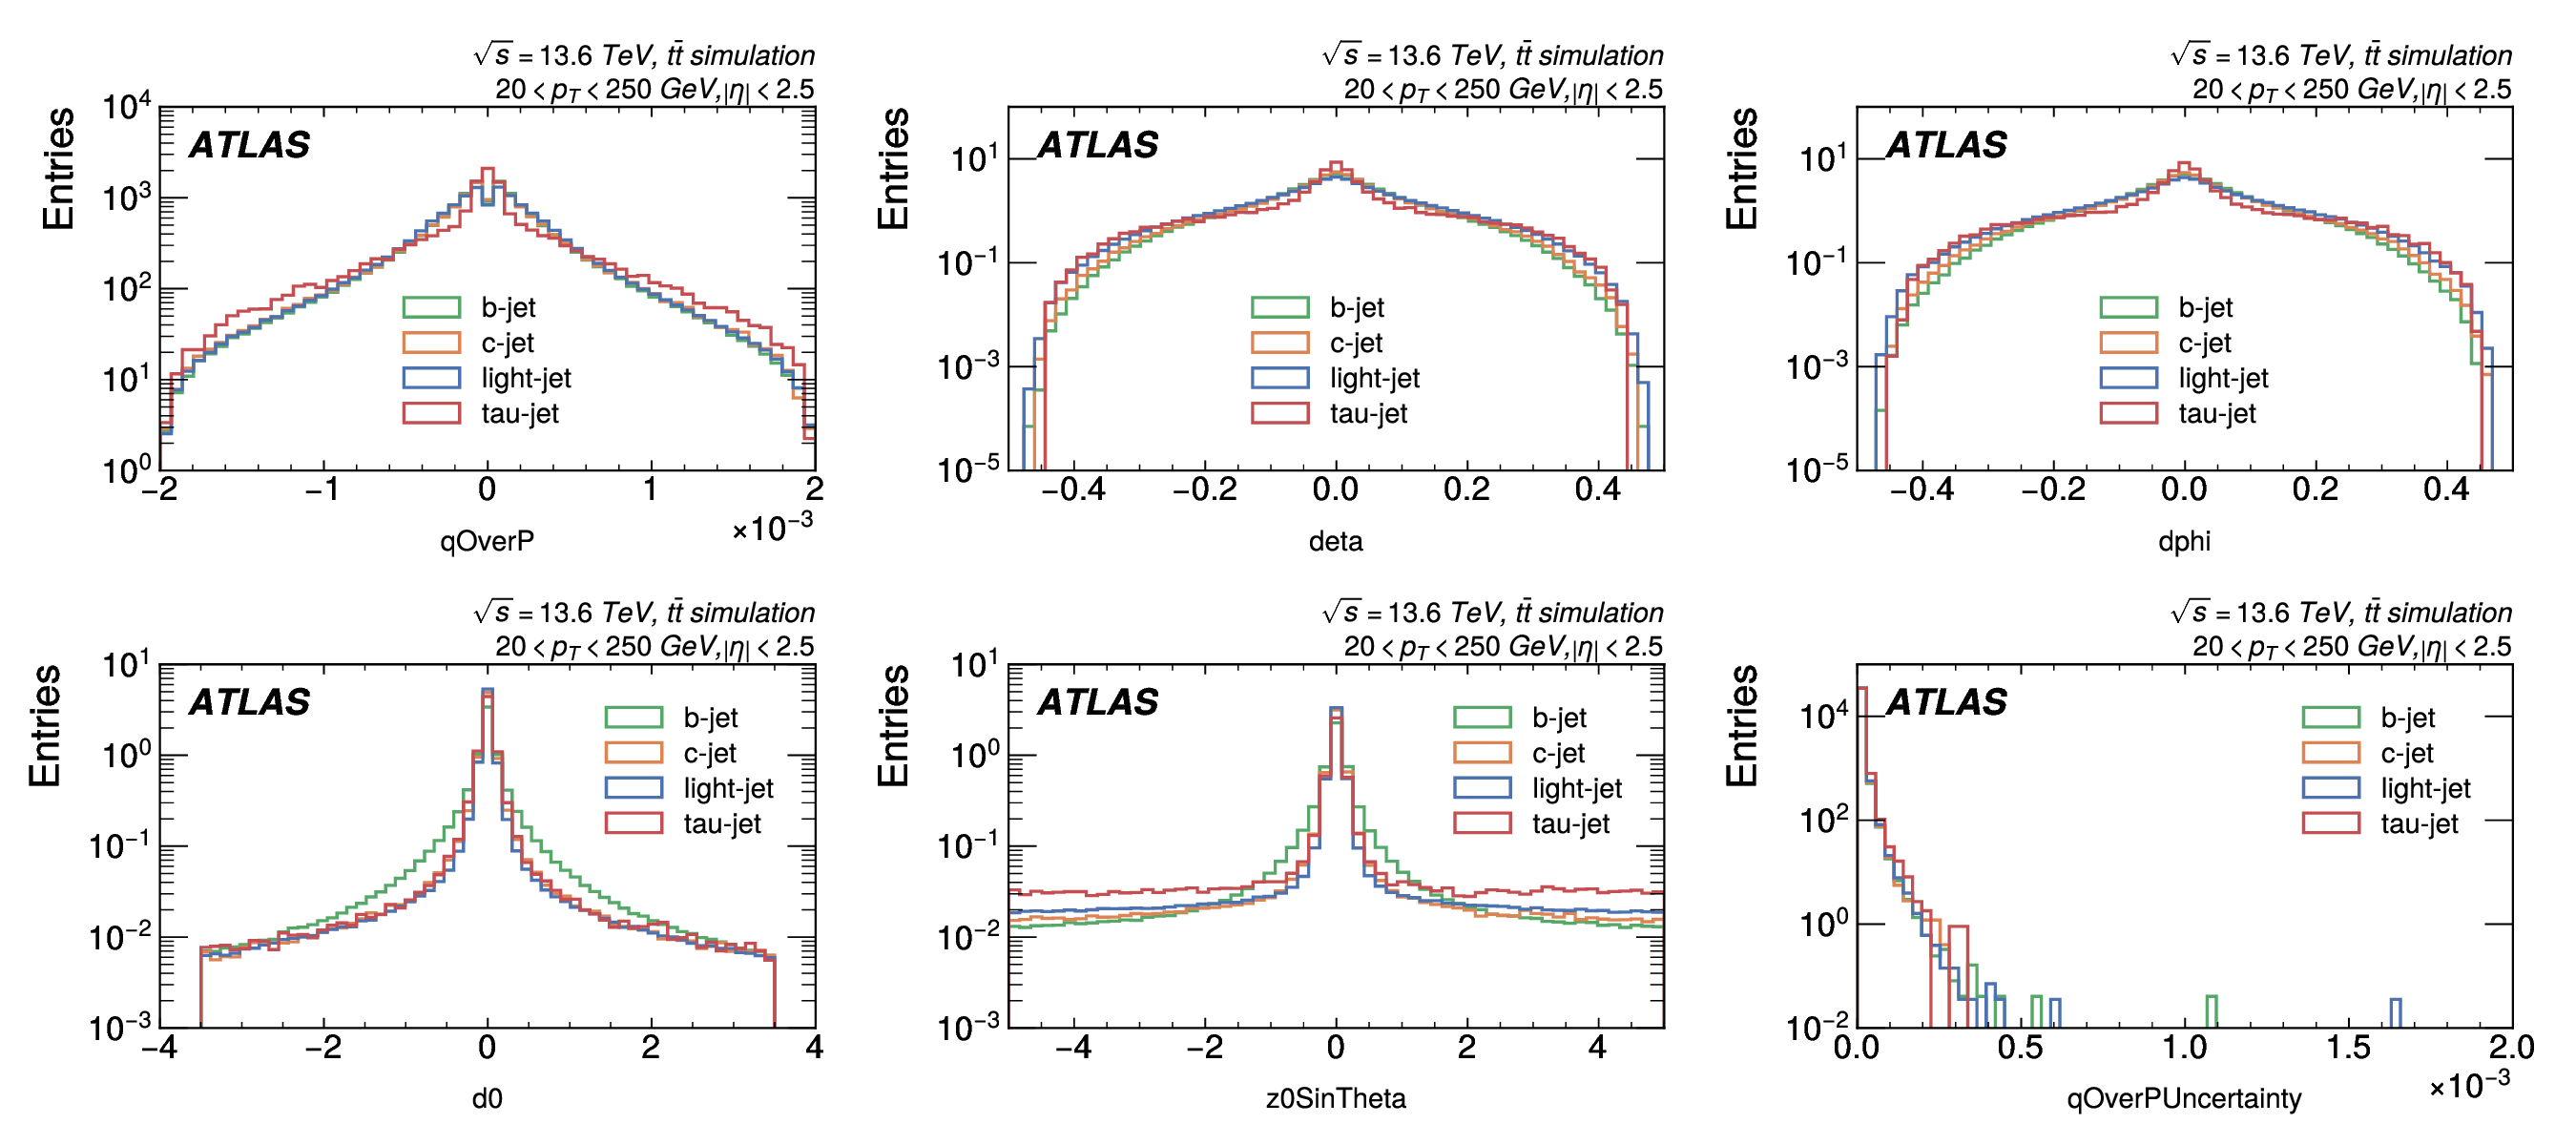
\includegraphics[width=\textwidth]{../../results/data_statistics/track_variables_page1.png}}\\
    \subfloat[\label{fig:lab_stat}]{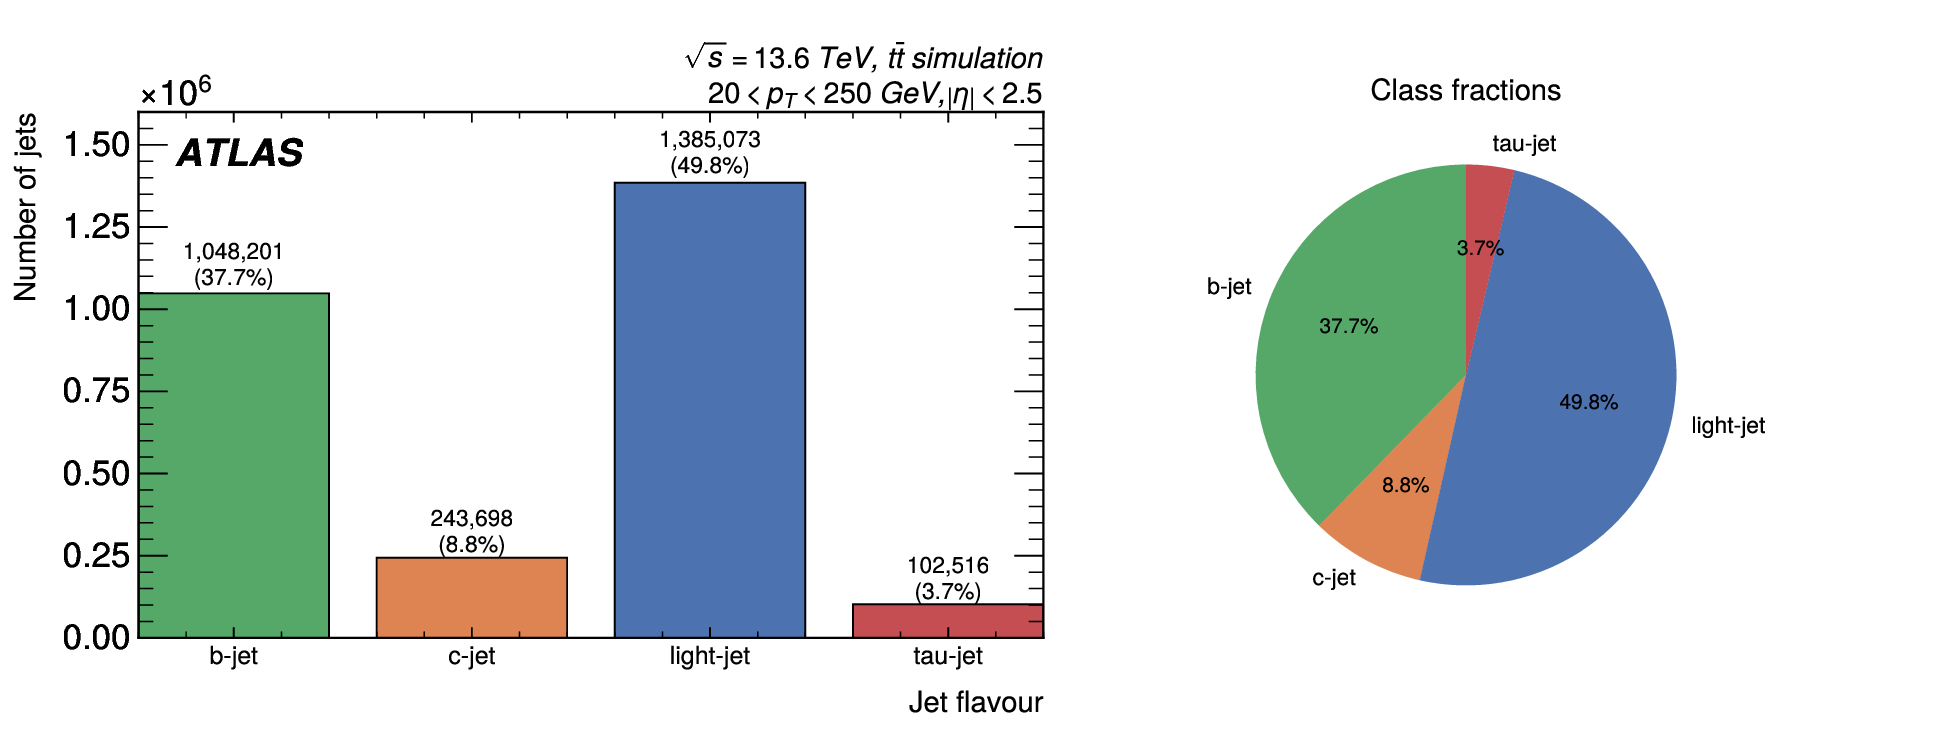
\includegraphics[width=\textwidth]{../../results/data_statistics/label_distribution.png}}
    \caption{Distribuzioni di alcune variabili di traccia (a) e distribuzione del sapore dei jet nel dataset (b).}
\end{figure}


\section{Architettura del Modello (\texttt{model.py})}

Il modello GN2 (classe \texttt{GN2}) elabora ciascun jet in quattro stadi sequenziali:

\begin{enumerate}[topsep=1pt, itemsep=0pt, parsep=1pt]
    \item \textbf{Inizializzatore per-traccia}: le variabili di jet vengono replicate e concatenate a quelle di traccia; un MLP a due strati mappa il vettore combinato in uno spazio di dimensione 64.
        \begin{center}
            \begin{tikzpicture}[scale=0.9]
                \draw[fill=green!20] (0,0) rectangle (1,2);
                \node at (0.5,-0.4) {$F_{jet}$};
                \node at (-0.4,1) {$B$};
                \draw[->, thick] (1.5,1.2) -- (2.5,1.2);
                \begin{scope}[xshift=3.5cm]
                    \draw[fill=green!20] (0,0) rectangle (1,2);
                    \draw[fill=green!10] (1,0) -- (1.7,0.5) -- (1.7,2.5) -- (1,2) -- cycle;
                    \draw[fill=green!30] (0,2) -- (1,2) -- (1.7,2.5) -- (0.7,2.5) -- cycle;
                    \node at (0.5,-0.4) {$F_{jet}$};
                    \node at (-0.4,1) {$B$};
                    \node at (1.5,0) {$T$};
                \end{scope}
                \node at (5.7,1.2) {$\oplus$};
                \begin{scope}[xshift=6.7cm]
                    \draw[fill=blue!20] (0,0) rectangle (2,2);
                    \draw[fill=blue!10] (2,0) -- (2.7,0.5) -- (2.7,2.5) -- (2,2) -- cycle;
                    \draw[fill=blue!30] (0,2) -- (2,2) -- (2.7,2.5) -- (0.7,2.5) -- cycle;
                    \node at (1,-0.4) {$F_{track}$};
                    \node at (-0.4,1) {$B$};
                    \node at (2.5,0) {$T$};
                \end{scope}
                \draw[->, thick] (9.9,1.2) -- (10.9,1.2);
                \begin{scope}[xshift=11.7cm]
                    \draw[fill=red!20] (0,0) rectangle (3,2);
                    \draw[fill=red!10] (3,0) -- (3.7,0.5) -- (3.7,2.5) -- (3,2) -- cycle;
                    \draw[fill=red!30] (0,2) -- (3,2) -- (3.7,2.5) -- (0.7,2.5) -- cycle;
                    \node at (1.5,-0.4) {$F_{jet}+F_{track}$};
                    \node at (-0.4,1) {$B$};
                    \node at (3.5,0) {$T$};
                \end{scope}
            \end{tikzpicture}
        \end{center}

    \item \textbf{Encoder transformer}: quattro strati con 8 teste di attenzione, embedding di dimensione 64 e feed-forward di dimensione 256, con pre-LayerNorm e connessioni residue; le posizioni di padding sono escluse tramite maschera booleana.
    
    \item \textbf{Attention pooling}: una query lineare appresa assegna pesi softmax a ciascun embedding di traccia, aggregandoli in una rappresentazione globale del jet di dimensione 128; questa scelta, rispetto al mean pooling, permette al modello di pesare esplicitamente le tracce più informative (e.g. quelle con parametri d'impatto più significativi).
    
    \item \textbf{Testa di classificazione}: un MLP ($128 \to 64 \to 32 \to 4$) produce le probabilità softmax per le quattro classi.
\end{enumerate}

Il modello contiene circa \textbf{230\,000} parametri addestrabili.
Le funzioni di attivazione disponibili sono ReLU, LeakyReLU, Sigmoid, Tanh e SoftPlus, con una scelta unica per tutto il modello; è inoltre possibile attivare il dropout.


\section{Addestramento (\texttt{train.py})}

Il training è interamente eseguito dalla funzione \texttt{train}, che inizializza:
\begin{itemize}[topsep=1pt, itemsep=0pt, parsep=1pt]
    \item \textbf{Loss}: cross-entropy a quattro classi per il task di classificazione del sapore del jet.
        I jet con etichetta $-1$ vengono ignorati tramite \texttt{ignore\_index=-1}.

    \item \textbf{Ottimizzatore}: tramite la funzione \texttt{get\_optimizer} è possibile scegliere tra AdamW, Adam e SGD.

    \item \textbf{Learning rate schedule}: warmup lineare da $10^{-7}$ a $5 \times 10^{-4}$ nel primo 1\% degli step, seguito da cosine annealing fino a $10^{-5}$.
\end{itemize}

Il ciclo di training è gestito da \texttt{run\_epoch}, lanciata sia per il training che per la validazione; nel solo caso di training esegue anche il backward pass.
Su GPU è attivata la mixed precision automatica (AMP); la norma del gradiente è tagliata a 1.0 per evitare instabilità.
Il miglior checkpoint per validation loss viene salvato su disco.

I principali iperparametri dell'addestramento sono riassunti nella Tabella~\ref{tab:hparams}.

\begin{table}[!ht]
    \centering
    \begin{tabular}{lc}
        \toprule
        Iperparametro & Valore \\
        \midrule
        Numero di epoche         & 21 \\
        Dimensione del batch     & 2048 \\
        Numero massimo di tracce & 40 \\
        Funzione di attivazione  & ReLU \\
        Dropout                  & No \\
        Ottimizzatore            & AdamW \\
        Learning rate iniziale   & $10^{-7}$ \\
        Learning rate di picco   & $5 \times 10^{-4}$ \\
        Learning rate finale     & $10^{-5}$ \\
        Weight decay             & $10^{-5}$ \\
        \midrule
        Dispositivo              & GPU (Tesla T4) \\
        Tempo di training        & circa 17 ore \\
        \bottomrule
    \end{tabular}
    \caption{Iperparametri usati nell'addestramento finale.}
    \label{tab:hparams}
\end{table}

\begin{figure}[!ht]
    \centering
    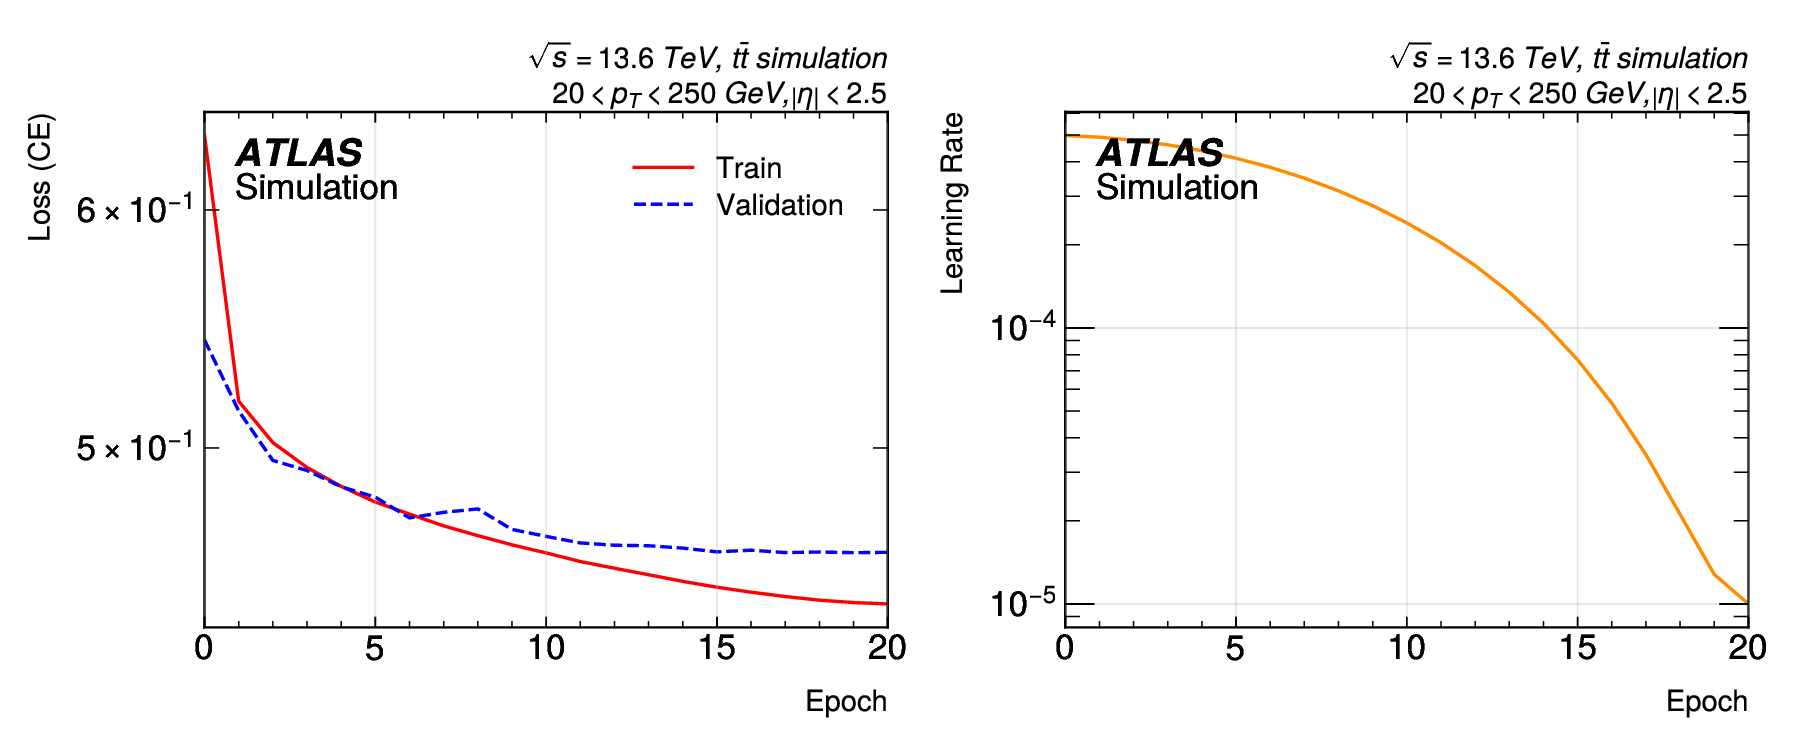
\includegraphics[width=0.9\textwidth]{../../results/learning_curves.png}
    \caption{Learning curves (training e validation loss) e profilo del learning rate schedule durante l'addestramento.}
    \label{fig:lc}
\end{figure}


\section{Valutazione (\texttt{evaluate.py})}

In fase di valutazione il miglior checkpoint viene caricato e applicato ai dati di test.
Vengono calcolate le metriche di classificazione e prodotte: la confusion matrix normalizzata, le distribuzioni degli score softmax e le curve ROC per i discriminanti di $b$- e $c$-tagging, definiti come:
\begin{equation*}
    D_b = \log\!\left(\frac{p_b}{f_c p_c + f_\tau p_\tau + (1-f_c-f_\tau) p_u}\right), \qquad
    D_c = \log\!\left(\frac{p_c}{f_b p_b + f_\tau p_\tau + (1-f_b-f_\tau) p_u}\right).
\end{equation*}

La pipeline produce i seguenti file di output:
\begin{itemize}[topsep=1pt, itemsep=0pt, parsep=1pt]
    \item \texttt{metrics.json}: accuratezza complessiva e, per ogni classe, precisione, recall e F1-score;
    \item \texttt{confusion\_matrix.pdf}: confusion matrix normalizzata (Fig.~\ref{fig:cm});
    \item \texttt{score\_distributions.pdf}: distribuzioni degli score softmax suddivise per sapore reale del jet (Fig.~\ref{fig:scores});
    \item \texttt{roc\_db.pdf}: curve ROC (rigetto del fondo vs. efficienza di $b$-jet) per il discriminante $D_b$ con $f_c = 0.20$, $f_\tau = 0.05$ (Fig.~\ref{fig:roc_db});
    \item \texttt{roc\_dc.pdf}: curve ROC analoghe per il discriminante $D_c$ con $f_b = 0.30$, $f_\tau = 0.01$ (Fig.~\ref{fig:roc_dc}).
\end{itemize}


\section{Risultati}\label{sec:risultati}

La valutazione delle prestazioni del modello viene condotta esclusivamente sul campione di test.
Le metriche globali ottenute sono riportate in Tabella~\ref{tab:metrics}.

\begin{table}[!ht]
    \centering
    \begin{tabular}{lcccc}
        \toprule
        Classe & Precisione & Recall & F1-score & Accuratezza globale \\
        \midrule
        b-jet       & 0.88 & 0.86 & 0.88 & \multirow{4}{*}{0.84} \\
        c-jet       & 0.54 & 0.16 & 0.24 & \\
        light-jet   & 0.83 & 0.96 & 0.89 & \\
        $\tau$-jet  & 0.69 & 0.58 & 0.63 & \\
        \bottomrule
    \end{tabular}
    \caption{Metriche di classificazione sul set di test. I valori si trovano nel file \texttt{metrics.json}.}
    \label{tab:metrics}
\end{table}

\subsection{Distribuzioni degli score di classificazione}

Le distribuzioni delle probabilità softmax $P(\text{classe})$ per ciascuna delle quattro categorie sono mostrate in Fig.~\ref{fig:scores}.
La distribuzione $P(b\text{-jet})$ mostra una separazione netta: i b-jet veri producono un picco pronunciato vicino a 1, mentre i light-jet dominano la regione a bassa probabilità.
Analoga separazione si osserva per $P(\text{light-jet})$.
Le distribuzioni $P(c\text{-jet})$ e $P(\tau\text{-jet})$ presentano una sovrapposizione maggiore tra le diverse classi, anticipando le difficoltà di classificazione di queste categorie.

\begin{figure}[!ht]
    \centering
    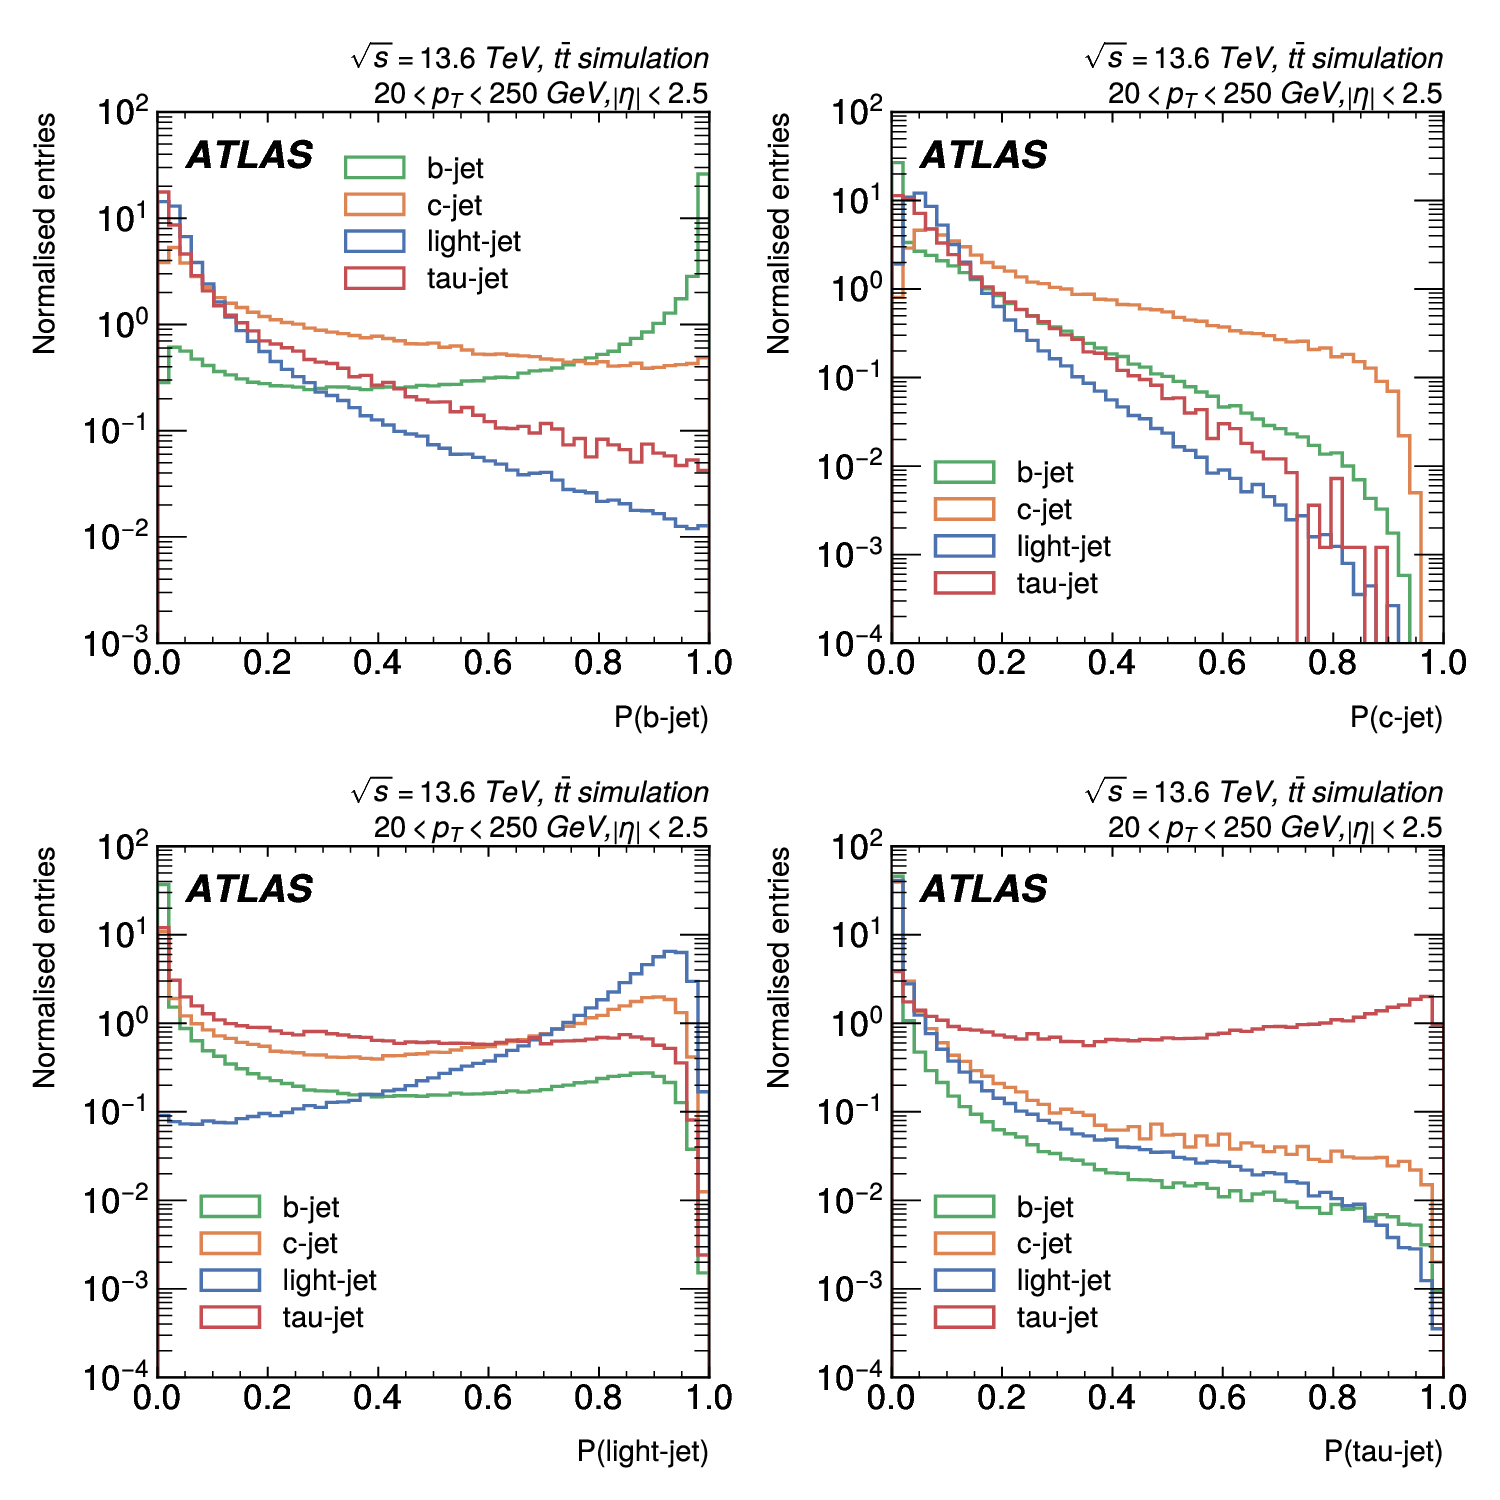
\includegraphics[width=0.8\textwidth]{../../results/eval/score_distributions.png}
    \caption{Distribuzioni normalizzate degli score softmax $P(\text{classe})$ per ciascuna delle quattro categorie, separate per sapore reale del jet.}
    \label{fig:scores}
\end{figure}

\subsection{Matrice di confusione}

La matrice di confusione normalizzata (Fig.~\ref{fig:cm}) riporta le probabilità di classificazione mediate per ciascuna coppia di sapore vero e predetto.
I light-jet mostrano le prestazioni migliori, con un'efficienza del 96\% e contaminazioni inferiori al 3\% verso tutte le altre classi.
I b-jet vengono identificati correttamente nell'87\% dei casi; la perdita principale avviene verso i light-jet (11\%).
La classificazione dei $\tau$-jet raggiunge un'efficienza del 58\%, con contaminazione prevalente di light-jet (32\%); tale comportamento riflette la somiglianza tra i decadimenti adronici del $\tau$ e i jet leggeri, specialmente a basso $p_T$.
La categoria più difficile rimane quella dei c-jet: l'efficienza è solo del 16\%, con la maggioranza classificata come light-jet (53\%).
Il marcato sbilanciamento del dataset (Fig.~\ref{fig:lab_stat}) contribuisce allo scarso risultato su $\tau$- e c-jet, poiché il modello ottimizza implicitamente le prestazioni sulle classi più abbondanti.

\begin{figure}[!ht]
    \centering
    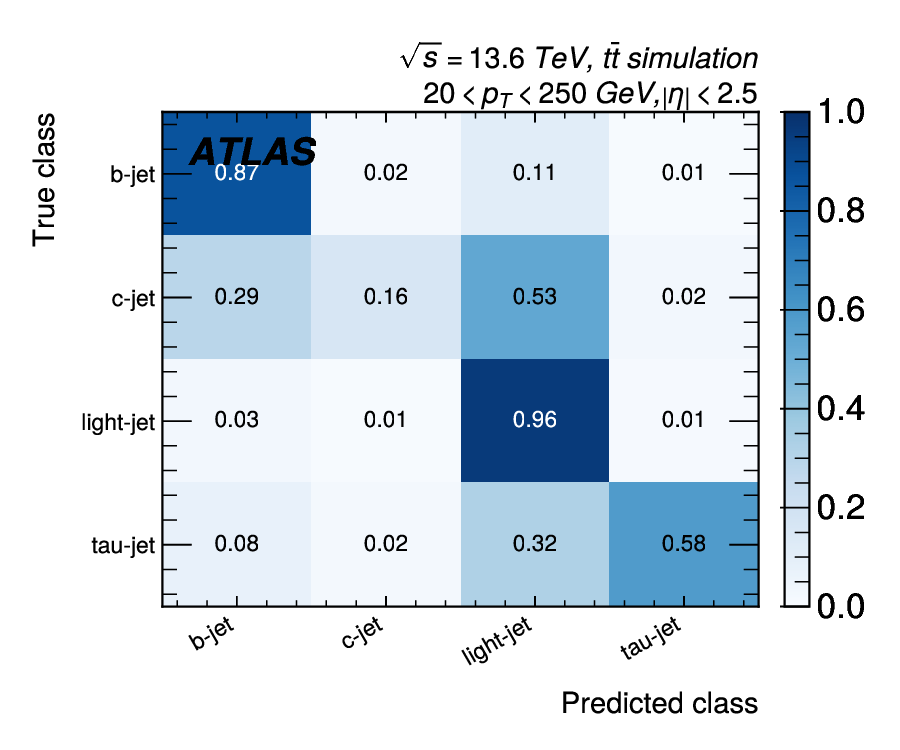
\includegraphics[width=0.65\textwidth]{../../results/eval/confusion_matrix.png}
    \caption{Matrice di confusione normalizzata sul test set.}
    \label{fig:cm}
\end{figure}

\subsection{Curve ROC}

Le curve ROC mostrano il rigetto del fondo in funzione dell'efficienza di b- (Fig.~\ref{fig:roc_db}) e c-tagging (Fig.~\ref{fig:roc_dc}).
Le curve ROC per il discriminante $D_c$ mostrano un regime di rigetto complessivamente più modesto, coerente con le difficoltà già evidenziate.
Al 70\% di efficienza di $b$-tagging il modello raggiunge rigetti di 700 (light-jet), 100 ($\tau$-jet) e 12 (c-jet), rispetto a 2000, 400 e 50 di GN2 (fattore $\sim3-4$).
Al 30\% di efficienza di $c$-tagging i rigetti scendono a 70 (light-jet), 12 (b-jet) e 4 ($\tau$-jet), contro 300, 20 e 60 di GN2 (fattore $\sim5-10$); il rigetto del $\tau$-jet pari a 4 indica un'assenza quasi totale di discriminazione in questo regime.

\begin{figure}[!ht]
    \centering
    \subfloat[]{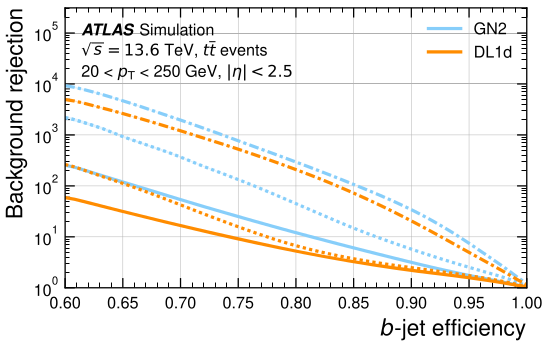
\includegraphics[width=0.45\textwidth]{../../results/article_b_jet.png}}
    \subfloat[]{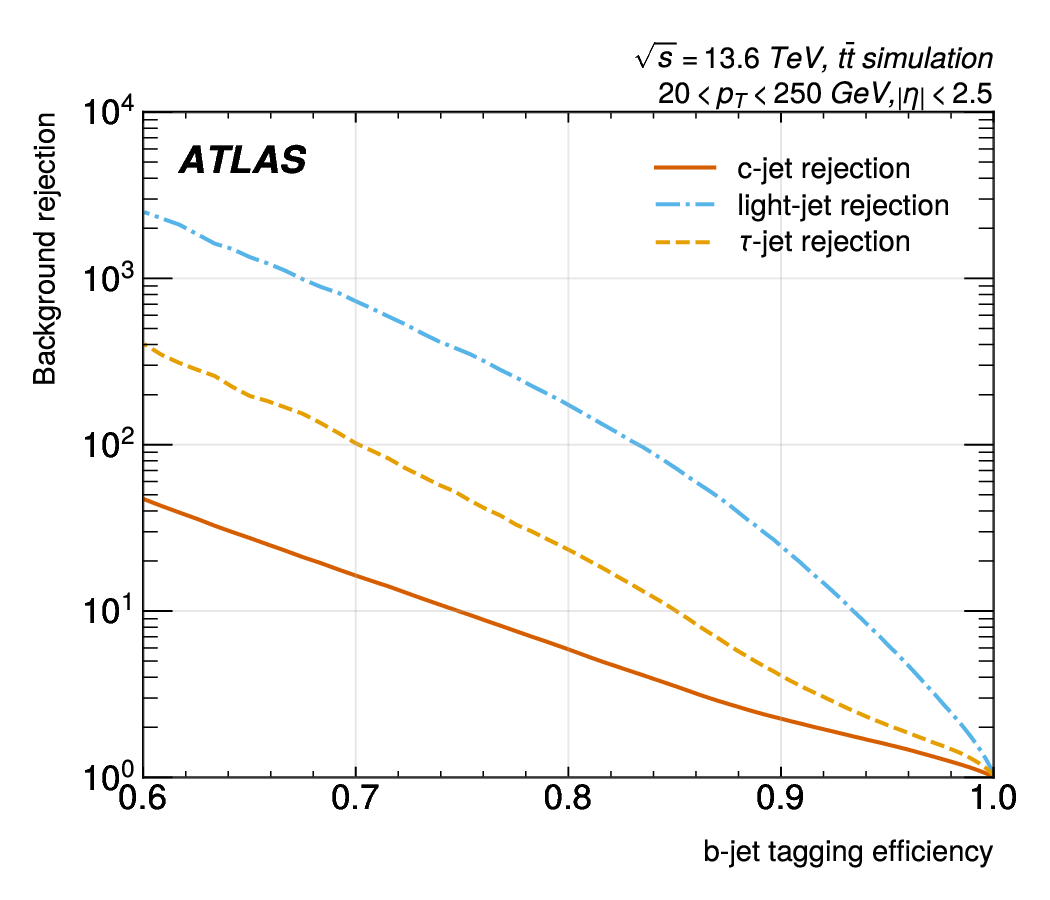
\includegraphics[width=0.45\textwidth]{../../results/eval/roc_db.png}}
    \caption{Curve ROC per il discriminante di $b$-tagging $D_b$: rigetto del fondo in funzione dell'efficienza di identificazione dei b-jet.
        A sinistra il risultato dell'articolo, mentre a destra il risultato con la nuova implementazione.}
    \label{fig:roc_db}
\end{figure}

\begin{figure}[!ht]
    \centering
    \subfloat[]{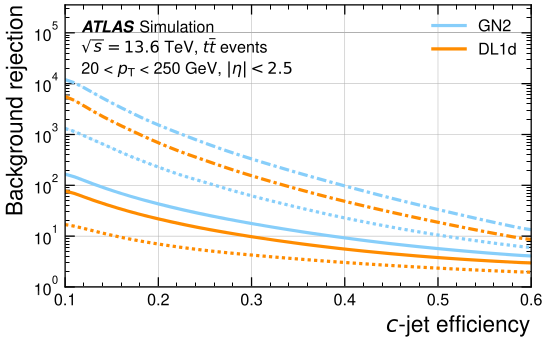
\includegraphics[width=0.45\textwidth]{../../results/article_c_jet.png}}
    \subfloat[]{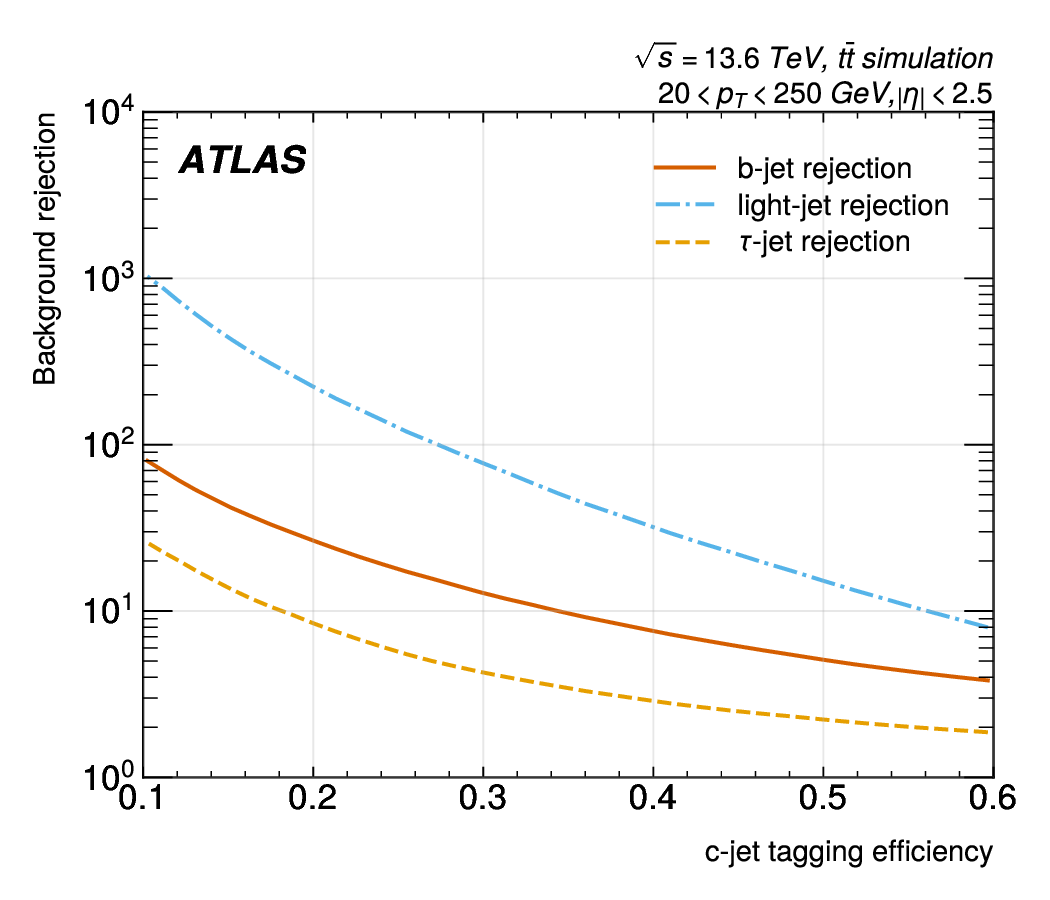
\includegraphics[width=0.45\textwidth]{../../results/eval/roc_dc.png}}
    \caption{Curve ROC per il discriminante di $c$-tagging $D_c$: rigetto del fondo in funzione dell'efficienza di identificazione dei c-jet.
        A sinistra il risultato dell'articolo, mentre a destra il risultato con la nuova implementazione.}
    \label{fig:roc_dc}
\end{figure}

\subsection{Riepilogo}

Nel complesso, il modello riproduce qualitativamente il comportamento atteso per un tagger basato su transformer: eccellente separazione dei light-jet, buone prestazioni per i b-jet, e difficoltà strutturale nel classificare c-jet e $\tau$-jet.
Le prestazioni quantitative sono inferiori al riferimento ATLAS di un fattore $\sim3-4$ per il $b$-tagging e di un fattore $\sim5-10$ per il $c$-tagging.
Tali differenze sono ragionevoli considerando che questa implementazione utilizza un sottoinsieme del dataset originale, non applica ottimizzazione sistematica degli iperparametri, oltre ad avere solo una frazione di parametri rispetto a GN2.

\begin{table}[!ht]
    \centering
    \begin{tabular}{cc}
        \begin{tabular}{lcc}
            \toprule
            Fondo & GN2 (ATLAS) & Questa impl. \\
            \midrule
            Jet-$c$     & 50   & 12  \\
            Jet leggero & 2000 & 700 \\
            Jet-$\tau$  & 400  & 100 \\
            \bottomrule
        \end{tabular}
        &
        \begin{tabular}{lcc}
            \toprule
            Fondo & GN2 (ATLAS) & Questa impl. \\
            \midrule
            Jet-$b$     & 20  & 12  \\
            Jet leggero & 300 & 70 \\
            Jet-$\tau$  & 60   & 4  \\
            \bottomrule
        \end{tabular}
    \end{tabular}
    \caption{Rigetto del fondo al 70\% di efficienza di $b$-tagging (sinistra) e al 30\% di efficienza di $c$-tagging (destra), confrontato con i valori ufficiali ATLAS per GN2.}
    \label{tab:rigetti}
\end{table}

\end{document}